\section{Wstęp}
\begin{frame}{Wstęp}
$m$ równań o m niewiadomych:
\begin{center}
$f_{i}(x_{1},\ x_{2},...,\ x_{j},...,\ x_{m})=0$; $i=1$, 2, $m... (*)$
$$
f\vec{(}\vec{x})=0
$$
\end{center}
Rozwiązanie układu: liczby $\alpha_{j}, j=1$, 2,..., $m$ takie że:
\begin{center}
$f_{i}(\alpha_{1},\ \alpha_{2},\ \alpha_{m})=0$; $i, j=1$, 2,..., $m$
\end{center}
Nie ma dobrych, ogólnych metod rozwiązania(*)
np. $m=2$
\end{frame}
\begin{frame}{Wstęp}
\begin{figure}[h]
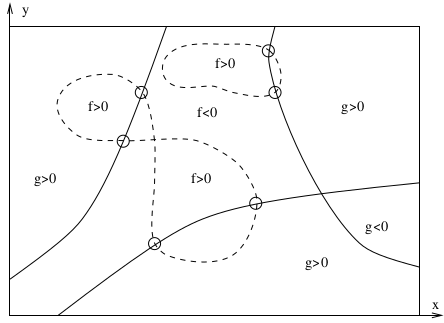
\includegraphics[width=0.75\linewidth]{img/9/9_1.png}
\end{figure}
$$
\left.\begin{array}{l}
f(x,\ y)=0\\
g(x,\ y)=0
\end{array}\right\} :
$$
 \end{frame}
\begin{frame}{Wstęp}
\begin{itemize}
\item kontury zerowe $\rightarrow$ podział płaszczyzny,
\item $\mathrm{f},\mathrm{g}-$dowolne $\Rightarrow$kontury bardzo złożone,
\item {\it liczba zer nie jest znana a priori},
\item dla $ x>2\rightarrow$hiperpłaszczyzny,
\item jak znaleźć punkty startowe?
\end{itemize}

\end{frame}